\section{Analítica Espacial}

\subsection{Métricas y Utilidad}

Este script calcula dos métricas principales para el manejo del tráfico: el 
Índice de Eficiencia y el Índice de Riesgo. El Índice de Eficiencia es una 
métrica que mide qué tan bien fluye el tráfico en un tramo específico, 
relacionando su capacidad de absorber un alto volumen de vehículos mientras 
mantiene una velocidad promedio óptima. Esto es muy útil para la toma de 
decisiones, ya que permite identificar qué avenidas están funcionando 
bajo su potencial y cuáles manejan un buen flujo de tráfico.

Por otro lado, el Índice de Riesgo analiza la seguridad de forma 
proporcional al volumen de tr\'afico. 
En vez de solo contar cuántos accidentes hay en una calle, este índice compara 
la cantidad de siniestros con el volumen total de tráfico que circula por el 
mismo lugar. 
Este enfoque es fundamental para analizar el peligro real de una ubicaci\'on.

\subsection{Lógica General}

\subsubsection*{Cargar Datos}

Importar las tablas de dimensi\'on 
\texttt{dim\_detector.csv} y
\texttt{dim\_ubicacion.csv}, y hechos
\texttt{fact\_medicion.csv} y
\texttt{fact\_siniestros.csv}.

\subsubsection*{Agregar Métricas de Tráfico}
\begin{itemize}[noitemsep]
    \item Agrupar la información de la tabla de mediciones utilizando el 
        identificador de cada detector.
    \item Calcular la velocidad media histórica y sumar el volumen total de 
        vehículos para cada detector.
\end{itemize}

\subsubsection*{Asignación Espacial de Siniestros}
\begin{itemize}[noitemsep]
    \item Iterar sobre cada uno de los siniestros registrados.
    \item Utilizar la fórmula de distancia Haversine para obtener la 
        distancia geográfica entre la ubicación del accidente y todos 
        los detectores de la ciudad.
    \item Identificar cuál es el detector más cercano al lugar del siniestro.
    \item Si la distancia al detector más cercano es inferior a 500 metros, 
        asignar ese siniestro a dicho detector.
    \item Agrupar los siniestros asignados y contabilizar el total por cada 
        detector, uniendo este resultado a los datos de tráfico previos.
\end{itemize}

\subsubsection*{Cálculo de Índices Normalizados}
\begin{itemize}[noitemsep]
    \item Normalizar los valores de volumen y velocidad, dividiendo cada 
        registro por el valor máximo histórico encontrado para llevarlos a una 
        escala estandarizada de 0 a 1.
    \item Calcular el Índice de Eficiencia multiplicando el volumen 
        normalizado por la velocidad normalizada, y ajustando a una escala 
        base 100.
    \item Calcular el Riesgo Inicial dividiendo la cantidad de siniestros 
        entre el volumen normalizado.
    \item Calcular el Índice de Riesgo final normalizando el riesgo inicial 
        contra el máximo riesgo detectado, ajustando nuevamente a una escala 
        base 100.
\end{itemize}

\subsubsection*{Exportar Resultados}
\begin{itemize}[noitemsep]
    \item Guardar la tabla final en el archivo 
        \texttt{tramos\_analitica\_2022.csv}. 
        El resultado generado es un archivo base que contiene un registro 
        único por cada detector (avenida/calle).
    \item Las columnas que se generan consolidan tanto la estadística cruda 
        (\texttt{cantidad\_siniestros}, \texttt{volumen\_total}, 
        \texttt{velocidad\_media}) como los dos nuevos indicadores creados 
        (\texttt{indice\_eficiencia}, \texttt{indice\_riesgo}).
\end{itemize}

Este archivo concluye la fase de procesamiento espacial y sirve como tabla 
maestra (o dimensión enriquecida) para alimentar los gráficos principales y 
mapas geográficos básicos en Power BI.

\subsection{Reporte}

\begin{figure}[ht]
    \centerline{
        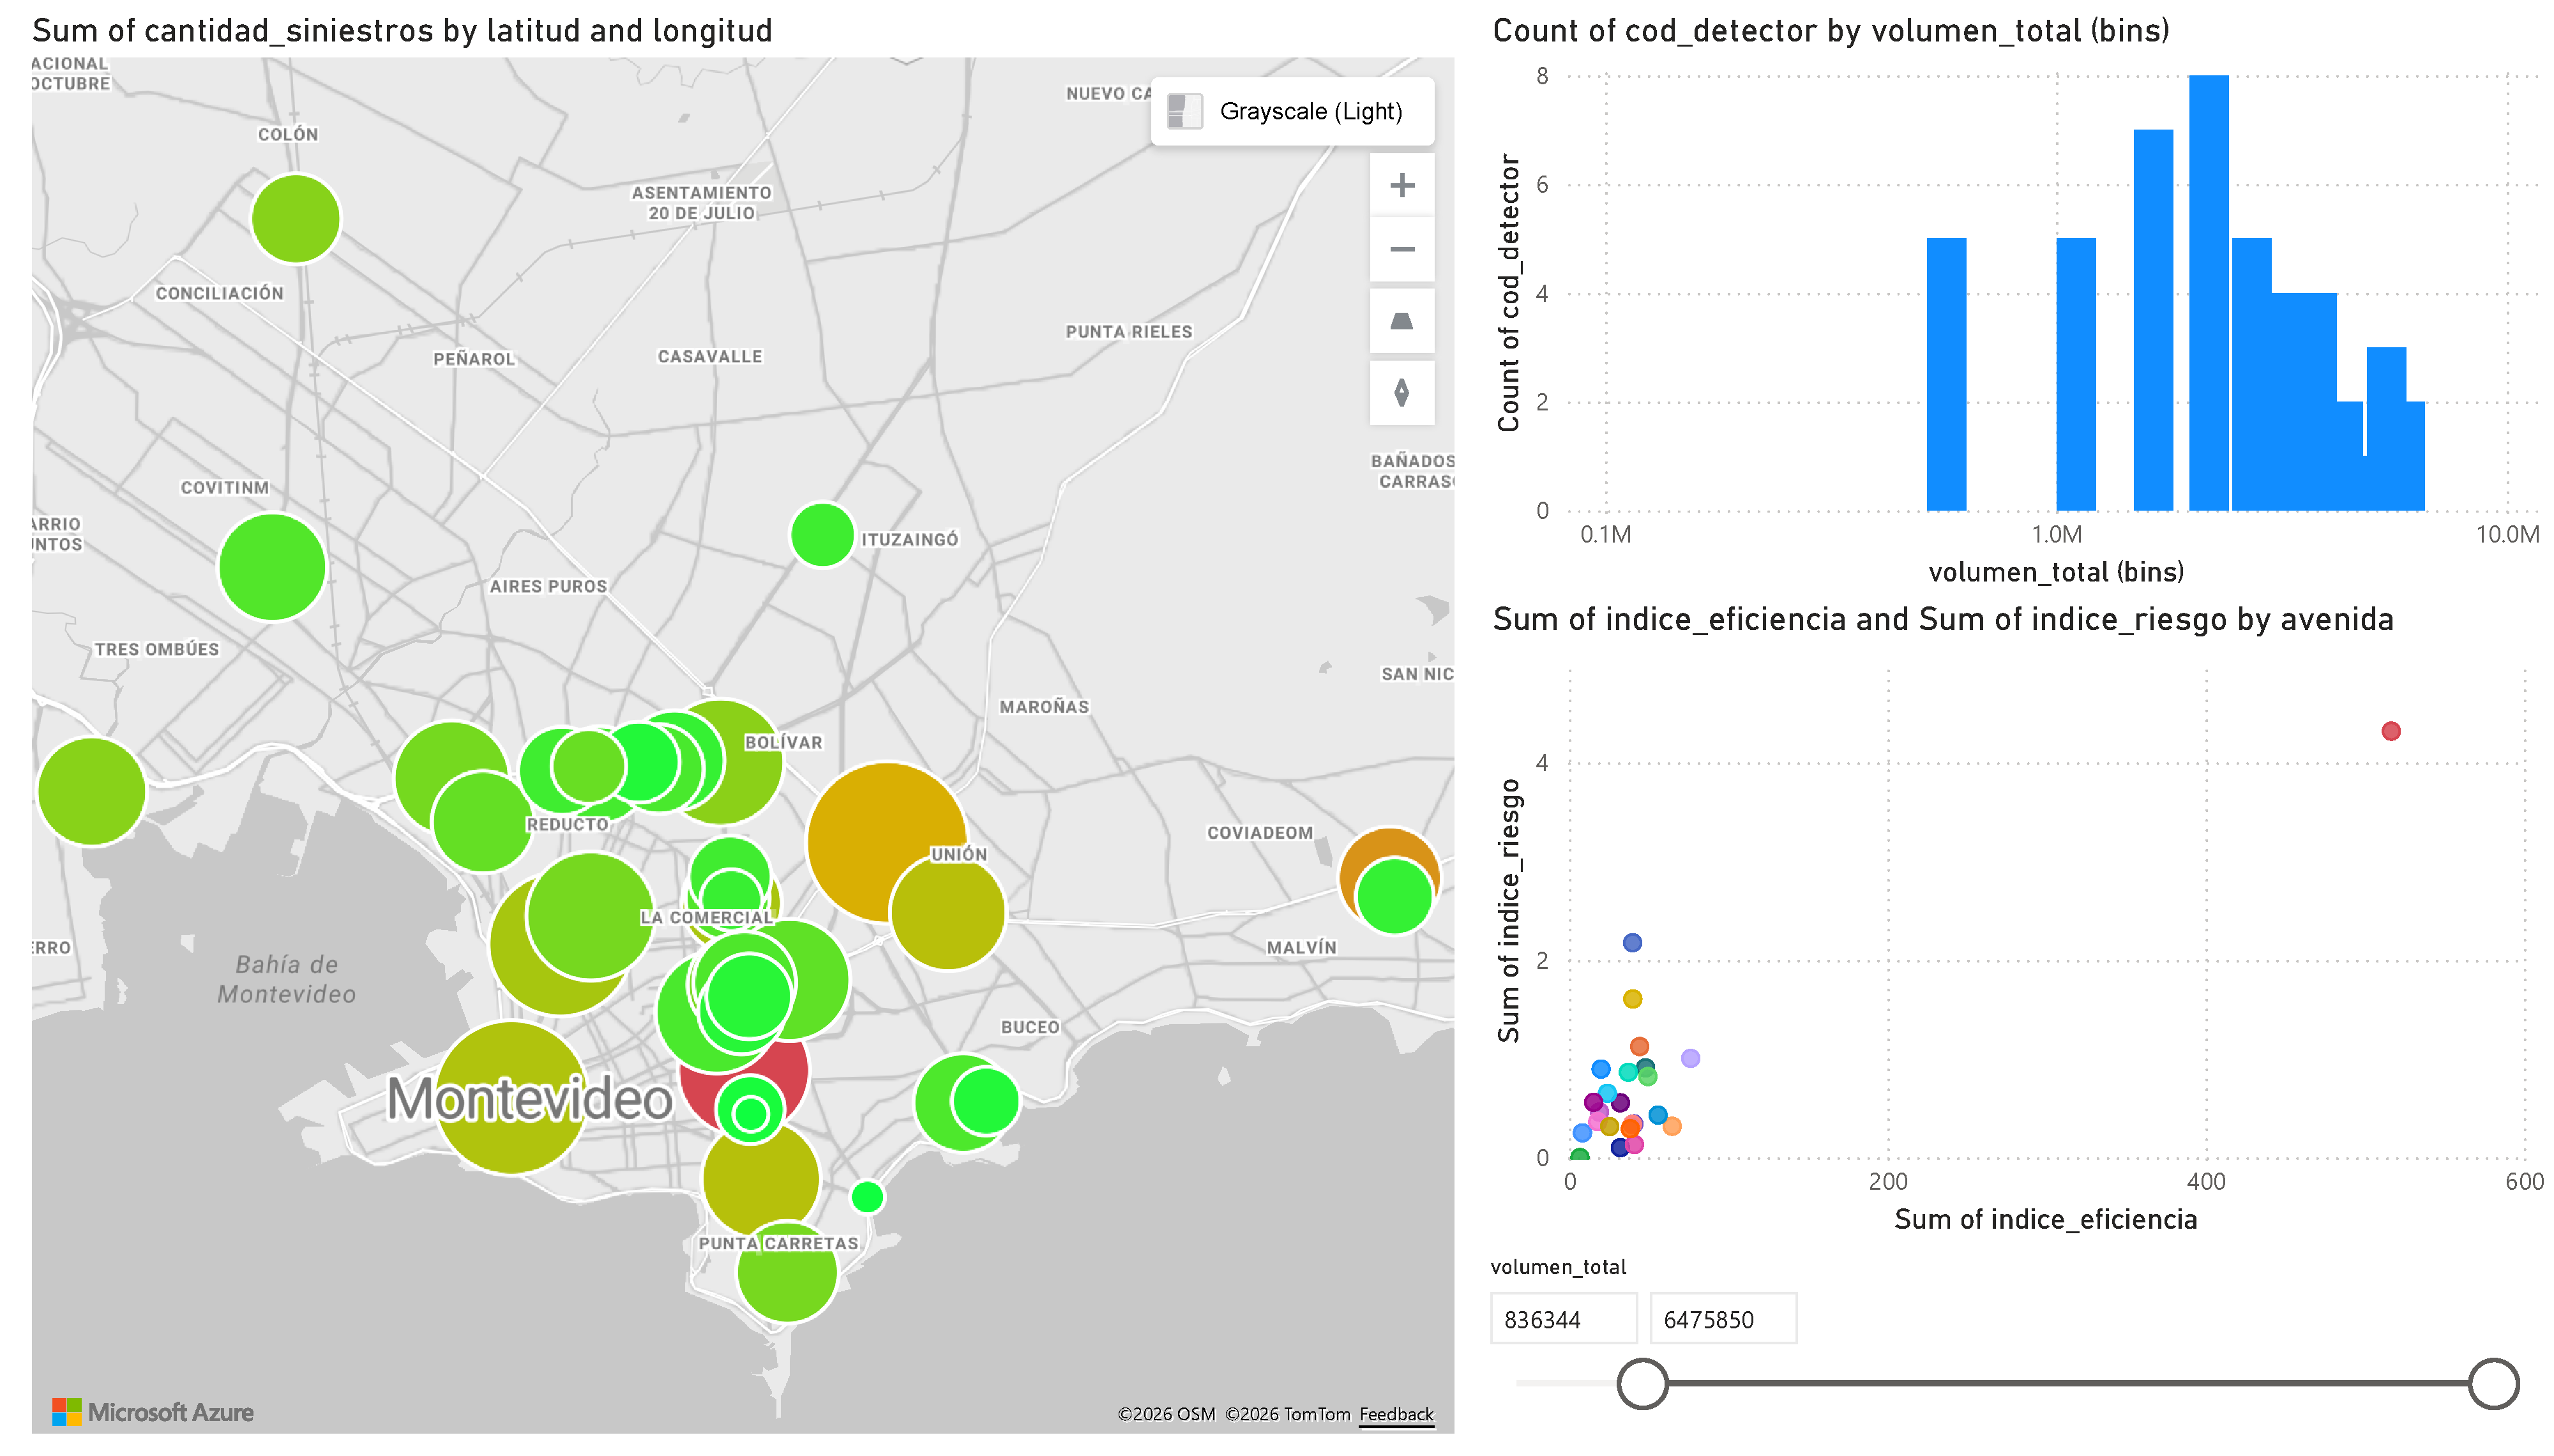
\includegraphics[page=1, scale=0.25]{graphics/reporte.pdf}
    }

    \caption{
        Reporte de las anal\'iticas iniciales: \\
        (\textbf{izquierda}) Mapa de cantidad de siniestros en cada zona 
            (detector). 
        (\textbf{arriba-derecha}) Histograma mostrando la distribuci\'on de 
            detectores seg\'un el volumen de autos medido. Notar que es una 
            escala logar\'itmica.
        (\textbf{abajo-derecha}) Slider para modificar los detectores mostrados 
            seg\'un el volumen de autos detectados.
    }

    \label{fig:reporte-analitica}

\end{figure}

Se debe notar que en \ref{fig:reporte-analitica}, el histograma tiene una escala 
logar\'itmica en el eje $x$ ya que encontramos varios outliers que mostraban 
un volumen peque\~no de autos detectados. Estos outliers no se ven en la 
gr\'afica gracias al slider que est\'a debajo de \'el. Este afecta a otros 
reportes, y esta repetido en ellos.
Se decide no mostrarlos ya que desv\'ian gravemente el resto de las m\'etricas 
calculadas, y probablemente no correspondan a datos correctos.


